%% Copyright (C) 2008 Johan Oudinet <oudinet@lri.fr>
%%
%% Permission is granted to make and distribute verbatim copies of
%% this manual provided the copyright notice and this permission notice
%% are preserved on all copies.
%%
%% Permission is granted to process this file through TeX and print the
%% results, provided the printed document carries copying permission
%% notice identical to this one except for the removal of this paragraph
%% (this paragraph not being relevant to the printed manual).
%%
%% Permission is granted to copy and distribute modified versions of this
%% manual under the conditions for verbatim copying, provided that the
%% entire resulting derived work is distributed under the terms of a
%% permission notice identical to this one.
%%
%% Permission is granted to copy and distribute translations of this manual
%% into another language, under the above conditions for modified versions,
%% except that this permission notice may be stated in a translation
%% approved by the Free Software Foundation
%%
\chapter{Solution to COCO 2018 keypoint task}
\label{sec:solution}
Similar to\cite{he2017mask, papandreou2017towards}, our algorithm adopts the top-downpipeline:
a human detector is first applied on the image to generate a set of human bounding-boxes and detailed localization
of the keypoints for each person can be predicted by a single-person skeleton estimator.
In addition, I use GAN to generate new train data. The extended train-set makes model more robust.

\section{Human detector}
We adopt the state-of-art object detector algorithms based on FPN\cite{lin2017feature}. ROIAlign from Mask RCNN\cite{he2017mask} is
adopted to replace the ROIPooling in FPN.
To train the object detector, all eighty categories from the COCO dataset are utilized during the training process but only the boxes of
human category is used for our multi-person skeleton task.

In our pipeline, we need a object detector which can find out the candidate human bounding-boxes as many as possible,
not the one which can predict the human bounding-boxes very accurately.
In another words, we need a object detector with high recall, not high precision.

\section{Human Pose Estimator}
Before starting the discussion of our algorithm, I first briefly review the design structure for the single person pose
estimator based on each human bounding box.
\subsection{Stacked Hourglass}
Stacked hourglass\cite{newell2016stacked}, which is a prevalent method for pose estimation,
stacks eight hourglasses which are down-sampled and up-sampled modules with residual connections to enhance the pose estimation performance.

The design of the hourglass is motivated by the need to capture information at every scale.
While local evidence is essential for identifying features like faces and hands, a final pose estimate requires a coherent understanding of the full body.
The person’s orientation, the arrangement of their limbs, and the relationships of adjacent joints are among the many cues that are best recognized at different scales in the image.
The hourglass is a simple, minimal design that has the capacity to capture all of these features and bring them together to output pixel-wise predictions.

Then the network is handled further by stacking multiple hourglasses end-to-end, feeding the output of one as input into the next.
This provides the network with a mechanism for repeated bottom-up, top-down inference allowing for reevaluation of initial estimates and features across the whole image.
The key to this approach is the prediction of intermediate heatmaps upon which a loss can be applyed.
Predictions are generated after passing through each hourglass where the network has had an opportunity to process features at both local and global contexts.
Subsequent hourglass modules allow these high level features to be processed again to further evaluate and reassess higher order spatial relationships.


\captionsetup[figure]{labelformat=empty}
\begin{figure}
  \centering
  \subfigure[One Hourglass]{
    \label{fig:subfig:a} %% label for first subfigure
    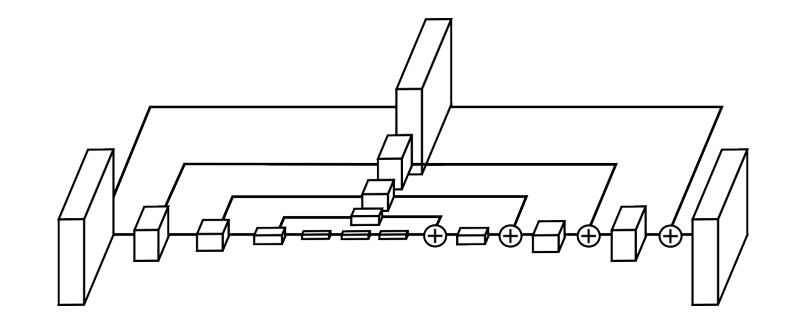
\includegraphics[width=6cm,height=4cm]{source/hourglass_single.png}}
  \hspace{1in}
  \subfigure[Stacked Hourglasses]{
    \label{fig:subfig:b} %% label for second subfigure
    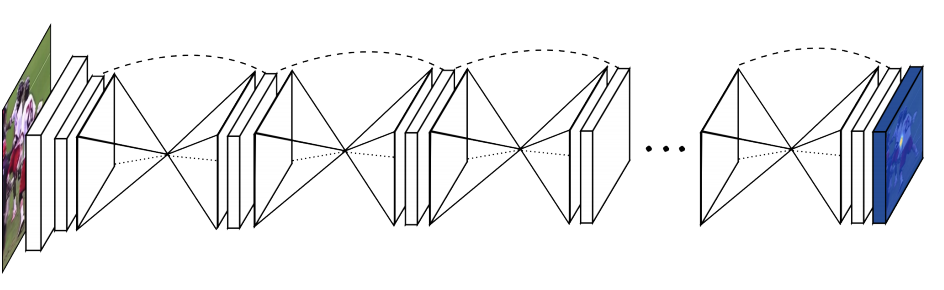
\includegraphics[width=6cm,height=4cm]{source/hourglass_total.png}}
  \caption{Figure 3: Hourglass Module. (a): The illustration of a single “hourglass” module. Each box in the figure corresponds
to a residual module. The number of features is consistent across the whole hourglass. (b) The illustration of multiple stacked hourglass modules
which allow for repeated bottom-up, top-down inference}
  \label{fig:1} %% label for entire figure
\end{figure}

\subsection{Cascaded Pyramid Network}
CPN\cite{chen2017cascaded} thought that stacking two hourglasses is sufficient to have a comparable performance
compared with the eight-stage stacked hourglass module. Hence, CPN involves two sub-networks: GlobalNet and RefineNet.

GlobalNet is based on the ResNet backbone. The last residual blocks of different conv features conv2∼5 are denoted as $C_{2}$, $C_{3}$, ..., $C_{5}$ respectively.
3 × 3 convolution filters are applied on $C_{2}$, ..., $C_{5}$ to generate the heatmaps for keypoints.
The shallow features like $C_{2}$ and $C_{3}$ have the high spatial resolution for localization but low semantic information for recognition.
On the other hand, deep feature layers like $C_{4}$ and $C_{5}$ have more semantic information but low spatial resolution due to strided convolution (and pooling).
Thus, usually an U-shape structure is integrated to maintain both the spatial resolution and semantic information for the feature layers.
GlobalNet can effectively locate the keypoints like eyes but may fail to precisely locate the position of hips.
The localization of keypoints like hip usually requires more context information and processing rather than the nearby appearance feature.

Based on the feature pyramid representation generated by GlobalNet, a RefineNet to explicitly address the
“hard” keypoints was attached.
In order to improve the efficiency and keep integrity of information transmission,
the RefineNet transmits the information across different levels and finally integrates the informations of different levels via upsampling
and concatenating as HyperNet\cite{kong2016hypernet}. In addition, more bottleneck blocks are stacked into deeper layers,
whose smaller spatial size achieves a good trade-off between effectiveness and efficiency.

\captionsetup[figure]{labelformat=empty}
\begin{figure}[htbp]
  \centering
  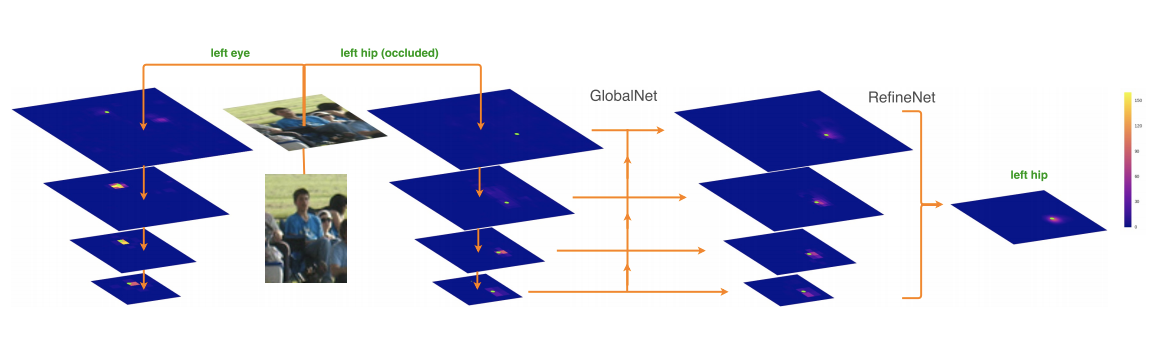
\includegraphics[width=16cm,height=4cm]{source/cpn.png}
  \caption{Figure 4: Cascaded Pyramid Network. Output heatmaps from different features. The green dots means the groundtruth location of keypoints.
  GlobalNet handles the easy case like left eye well.
  RefineNet integrates more information to locate the hard case, like occluded left hip.}
\end{figure}

\subsection{Our Pose Estimator}
Motivated by the works\cite{newell2016stacked, chen2017cascaded} described above, we propose an effective and efficient network to address the problem of pose estimation.
As shown in Figure 5, our model is a multi-stage network.

\captionsetup[figure]{labelformat=empty}
\begin{figure}[htbp]
  \centering
  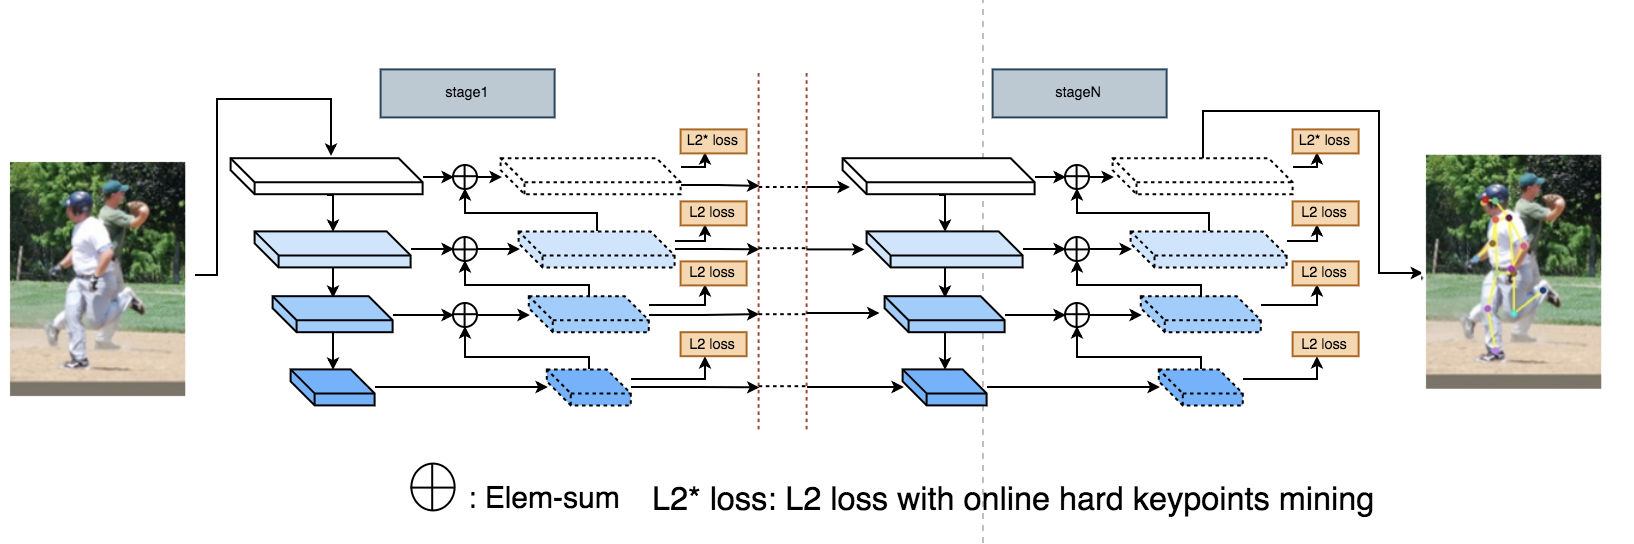
\includegraphics[width=16cm,height=6cm]{source/multi-stage.png}
  \caption{Figure 5: Our multi-stage network. Each stage is a U-shape structure based on the variant resnet.
  Different stages focus on diffferent poses. The later stage studies the harder pose.}
\end{figure}

\subsubsection{Singe Stage}

\textbf{Every single stage is a U-shape structure}.

As we all known, classification task needs semantic information and spatial information is necessary for location task.
The keypoint task contains both classification and location task because we need to not only classifer different body parts but also give precise coordinates.
In other words, we need both semation information and spatial information.
This is why we adopt U-shape structure.

The U-shape structure is based on the ResNet backbone. The last residual blocks of different conv features conv2∼5 are denoted as $C_{2}$, $C_{3}$, ..., $C_{5}$ respectively, like the cuboids with full line in Figure 5.

In the down-sampling procedure, the resolution of feature map zooms out 5 times(conv1~5).
For example, if the size of input was $256*192$, the lowest resolution could be $8*6$.
Hence, every pixel in $8*6$ size feature map owns a huge receptive field and the $8*6$ size feature map has high-dimensinal semantic information but lacks spatial information.
On the contrary, the high solution feature map has more spatial information and less semantic information.

And then the up-sampling procedure will be passed.
With a coarser-resolution feature map, we upsample the spatial resolution by a factor of 2 (using bilinear interpolation for accuracy).
The upsampled map is then merged with the corresponding down-sampling map (which undergoes a $1*1$ convolutional layer to reduce channel dimensions) by element-wise addition.
This process is iterated until the finest resolution map is generated.
To start the iteration, we simply attach a $1×1$ convolutional layer on $C_{5}$ to produce the coarsest resolution map.
Afterwards, we append a $1*1$ convolution on each merged map to generate the final feature map, which is to reduce the aliasing effect of upsampling and to reduce the dimensions(numbers of channels) to 256.
This final set of feature maps is called $\{P_{2}, P_{3}, P_{4}, P_{5}\}$, corresponding to $\{C_{2}, C_{3}, C_{4}, C_{5}\}$
that are respectively of the same spatial sizes.

Finally, every final feature maps will pass 2 Conclusion layes($3*3$ and $1*1$) to generate the 17 dimensinal heapmaps.

\captionsetup[figure]{labelformat=empty}
\begin{figure}[htbp]
  \centering
  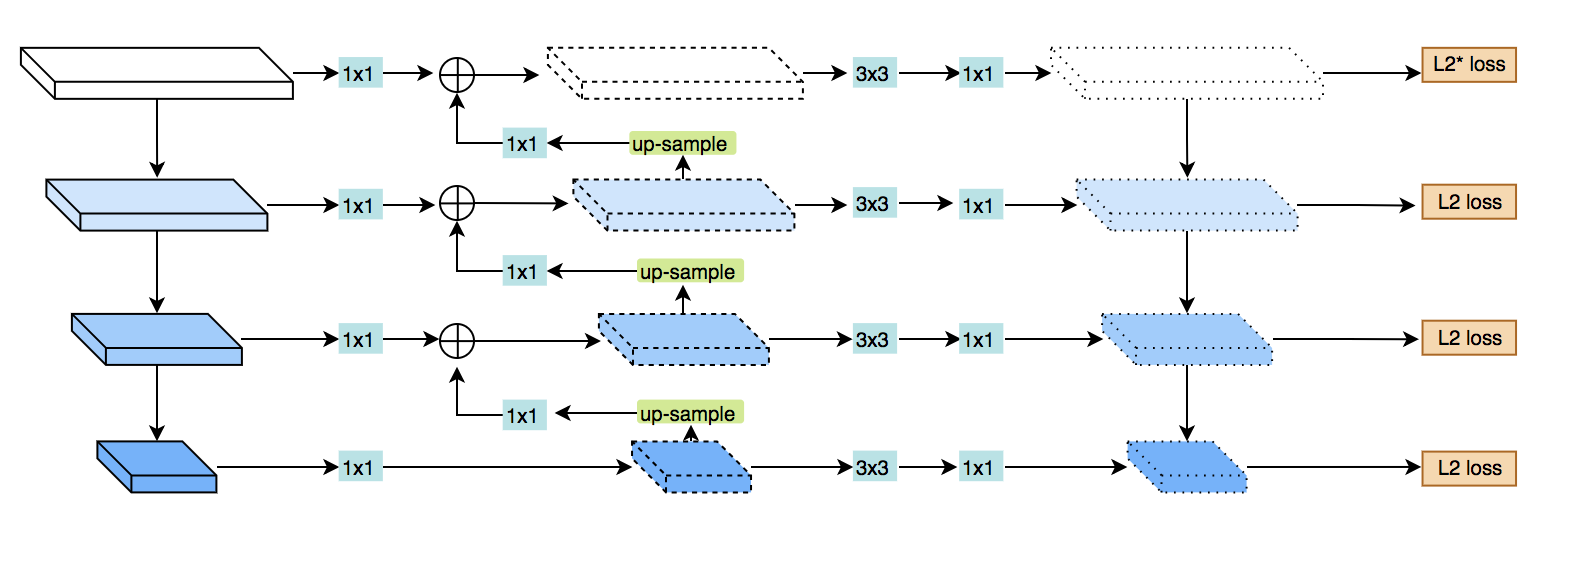
\includegraphics[width=16cm,height=6cm]{source/single-stage.png}
  \caption{Figure 6: Details of U-shape structure for single stage}
\end{figure}

\textbf{Intermediate Supervision}

The U-shape architecture provides a top-down, bottom-up inference allowing for generation of heatmaps with different resolution.
Hence, we can apply a loss upon the prediction of intermediate heatmaps.
Predictions are generated after passing through each final feature map $\{P_{2}, P_{3}, P_{4}, P_{5}\}$ where the network has had an opportunity to process features at both local and global contexts.
This is similar to other pose estimations methods that have demonstrated strong performance with multiple iterative intermediate supervision\cite{wei2016convolutional, carreira2016human}.

\textbf{Every single stage is a variant Resnet}.

Nowadays, Resnet\cite{he2016deep} is the most common basemodel in all kinds of Computer-vision task.
The core idea of Resnet is the residual learning which can avoid the gradient vanishing effectively.
Hence, Resnet can be designed very deeply, like resnet50, resnet101, resnet152.
\[ y = F(x, \{W_{i}\}) + x ...................(2)\]
Eqn 1 explained the residual learning. Here $x$ and $y$ are the input and output vectors of the layers considered.
The function $F(x, \{W_{i}\})$ represents the residual mapping to be learned.

\captionsetup[figure]{labelformat=empty}
\begin{figure}
  \centering
  \subfigure[One Hourglass]{
    \label{fig:subfig:a} %% label for first subfigure
    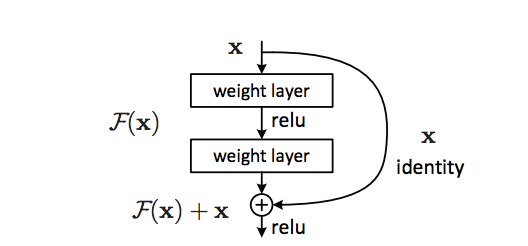
\includegraphics[width=6cm,height=4cm]{source/residual_learning.png}}
  \hspace{1in}
  \subfigure[Stacked Hourglasses]{
    \label{fig:subfig:b} %% label for second subfigure
    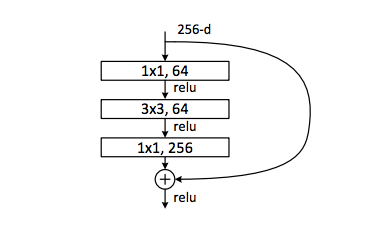
\includegraphics[width=6cm,height=4cm]{source/residual_block.png}}
  \caption{Figure 7: Residual block. (a): The residual-block for residual learning. (b) The realization of residual block in Resnet50, 101, 152}
  \label{fig:1} %% label for entire figure
\end{figure}

As mentioned before, keypoint detection task needs both semantic information and spatial information.
But are they same important?
We did several experiments using res50, res101 and res152 as single stage network respectively.
Single stage has mAp $73.3\%$ with res50, $73.7\%$ with res101, $73.8\%$ with res152.
Compared with res50, res101 got $0.4\%$ mAp gain.
However, res152 only got $0.1\%$ more mAp than res101.
As shown in Figure 8, the difference better res50, res101 and res152 is the number of residual blocks in Conv4.
Conv4 learns more semantic information, and increasing the complexity in Conv4 doesn't seem to work.
Hence, we got a conclusion: \textbf{for keypoint detection task, spatial information is more important than semantic information.}

Then we designed a variant Resnet.
In normal Res101, The number of residual block of different Conv stage is $\{3, 4, 23, 3\}$.
Our variant Res101 adopts $\{4, 8, 16, 3\}$, which maintains same FLOPs as normal Res101 but adds more complexity in Conv2 and Conv3.
And it has $74.1\%$ mAp, more $0.4\%$ mAp than normal Res101 in the case of the same complexity.


\captionsetup[figure]{labelformat=empty}
\begin{figure}[htbp]
  \centering
  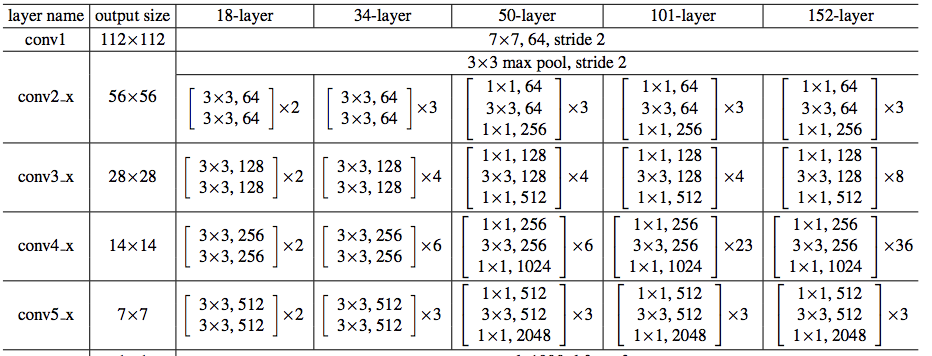
\includegraphics[width=16cm,height=6cm]{source/resnet.png}
  \caption{Figure 8: Different Resnet Architectures}
\end{figure}

\subsubsection{Multi-Stage}

\textbf{Hard pose samples are really rare.}

In keypont detection, the object keypoint similarity (OKS), seen in Eqn 1, is required to define positives and negatives.
At beginning, we trained a one-stage model and did the failure case analyse.
We found that most normal poses can be handled well, but a few hard poses like Parkour or playing skateboard are detected with low OKS.
Two main factors are responsible for this: 1)hard poses are inherently challenging  and 2) overfitting for normal poses during training, due to lack of hard poses.
Hence, motivated by cascade r-cnn\cite{cai2017cascade}, a multi-stage keypoint estimator architecture is proposed to the second factor.
It consists of a sequence of single estimator as mentionde before trained with increasing OKS thresholds, to be sequentially more selective against close false positives.
The estimators are trained stage by stage, leveraging the observation that the output of a estimator is a good distribution for training the next higher quality estimator.

For example, if we take 3 stage architecture, the input of first stage are all samples,
the input of second stage are those whose OKS is smaller than 0.8 accroding to the output of first stage,
and the input of third stage are those whose OKS is smaller than 0.6 accroding to the output of second stage.
The resampling of progressively guarantees that the later stage pays morr attention to the harder pose, reducing
the overfitting problem.

\textbf{We don't need pre-train a model using Imagenet.}

Since R-cnn\cite{girshick2014rich}, we always initialize our basemode by the parameters pre-trained on Imagenet, then finu-tune the model by the specific dataset.
It seems like a common sense, which no one doubts.
Howerver, is that really suitable for keypoint detection?
\textbf{Our answer is no.}

We did several comparative experiments, Table 2 shows the results.

\captionsetup[table]{labelformat=empty}
\begin{table}[!hbp]
  \centering
  \begin{tabular}{|c|c|c|c|c|}
  \hline
            & 3xres50 & 4xres50 & 2xres101 & 2xresInc101  \\
  \hline
  Initialization using Gaussian & 77.5 & 77.8 & 77.0 & 77.5 \\
  \hline
  Initialization using pre-trained parameters & 76.9 & 77.0 & 76.2 & 76.9 \\
  \hline
  \end{tabular}
  \caption{Table 2: comparative experiments results for initialization problem.}
\end{table}

We can find that initialization using Gaussian is generally better than initialization using pre-trained parameters.
Hence, we get a conclusion: \textbf{Imagenet task is a pure classification task, which prefers to semantic information.
This is why using parameters pre-trainded on Imagenet for initialization results in a worse performance.
The best solution is that we pre-train our model in a large auxiliary keypint dataset.}





%%% Local Variables:
%%% mode: latex
%%% TeX-master: "rapportM2R"
%%% End:
